\chapter{DNS}
\label{chp:dns}

\section{Introduction}

\Gls{dns} is an important part for the internet. It is a system of distributed databases which contains the information about all the domains. In the mid and late 1980s did the previous system, \texttt{HOST.TXT}, encounter problems \cite{Mockapetris:1988:DDN:52324.52338} which lead to the creation and standardizing called \Gls{dns}. Since that has the \Gls{dns} system been updated and configured many times. It needed to be able maintain a fast response time as the database grew larger, this was solved by using a hierarchical set up. This means that each server only has a limited information and sends the request to a new server until it reaches the correct server. It started with one root server, which has expanded to 13 today. The each layer of the hierarchy is called a zone, and it delegates the responsibility for underlying zones delimited by the \texttt{dot} in the request name \fref{fig:namespace}.

\begin{figure}
\centering
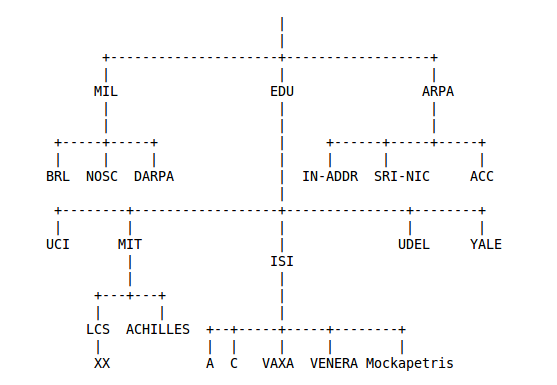
\includegraphics[scale=0.5]{figs/namespace_example.png}
\caption{\label{fig:namespace}Example of name spaces of a root with MIL, EDU and ARPA as immediate subdomains. Each leaf is a domain \citep{mockapetris1987domain}.}
\end{figure}



\section{Structure}
The data in the databases are called \Gls{rr} and contains the information about what the server do with the request. It has the following fields \cite{mockapetris1983domain}:
\begin{itemize} 
\item NAME -- the owner name of the record.
\item TYPE -- what type of record this is, name-to-IP (A) or IP-to-name (PTR).
\item CLASS -- define the class of the record, usually \texttt{IN} for internet. It is not widely use and not important for this paper.
\item TTL -- an integer which says how long the record should be cached by the server receiving the response.
\item RDLENGTH -- Specifies the length of the payload in number of octets. One octet is one octet of bits which corresponds to one character
\item RDATA -- the payload of the record. The format and length varies depending on the TYPE and CLASS of the \Gls{rr}.
\end{itemize}

\gls{dns} was first implemented with around 15 different \gls{rr} TYPE, which has now increased to over 30 \cite{farnham2013detecting} as a result of the development of the internet. The most notable values for TYPE are:

\begin{itemize}
\item A -- the payload will contain the ipv4 address of the hostname requested. This is the most used TYPE
\item AAAA -- contains the ipv6 address of the hostname.
\item CNAME -- canonical name, respond with the correct alias of the hostname.
\item MX -- the mail exchange for the domain
\item TXT -- a text response with large payload, can be used in many ways and are an important type in \gls{dns} tunneling.
\item PTR -- pointer record. Used to map a hostname to an IP-address, commonly known as a reverse lookup.
\item NS -- authoritative name server for the domain
\end{itemize}

The 'A' type \gls{rr} for telenor.no at the name server will look something like this:

\begin{table}
\centering
\begin{tabular}[c]{|l|l|}
\hline
\textbf{Field} & \textbf{Value} \\ \hline
NAME & telenor.no \\ \hline
TYPE & A \\ \hline
CLASS & IN \\ \hline
TTL & 300 \\ \hline
RDLENGTH & 15 \\ \hline
RDATA & 153.110.156.145 \\ \hline

\end{tabular}
\caption{\label{tab:rrexample}Example of \gls{rr} for telenor.no}
\end{table}


\section{How it works}
To explain of \Gls{dns} works is an example the easiest way

When a request goes through \Gls{dns} it starts in the root zone, where it sent down the hierarchy to the \texttt{.no} zone.



Normally a \Gls{dns} server in an enterprise does not send requests directly to the internet, but use an internal \Gls{dns} server instead. If you are the owner of the authoritative server for a domain, you can control the responses. This is what a \Gls{dns} tunnel exploits, which will be explained more in the next section. 





 